% Changed: recover service economics, complementary breadth and mechanism-led evaluation.
% Protected: all measurement clocks, cohort distinctions and negative outcomes.
% Meaning-Check: PRESERVED
% Risk-Flags: none
\section{Evaluation}
\label{sec:evaluation}
We test one service-level claim: governing the layout, evidence and publication of a reusable prefix can produce useful, amortized service state. The evidence proceeds from template economics and full-cost execution to behavior, governance, scale and operating conditions. Each regime retains its own source set, qualification unit and clock.

\subsection{Workloads, Controls, and Units}
\label{sec:protocol}
The primary cohort contains three HotpotQA and three RepoBench sources, chosen by frozen hash order after excluding 567 previously used sources~\cite{hotpotqa2018,repobench2024}. Reading-comprehension data come from the LongBench collections~\cite{longbench2024}. Each source defines a ten-tenant, ten-round template with three recurring query wrappers and changing private metadata. This is an explicitly repeated authorized directory, not a measured production query distribution.

We run Qwen3-8B, Mistral-7B-Instruct-v0.3, and Llama-3.1-8B-Instruct~\cite{qwen32025,mistral2023,llama32024}. Both policies have the same 16K window, retained task content, greedy decoding, fixed seed, request order, and two-request wave clock. HotpotQA has a 128-token generation budget and RepoBench 384. \emph{Raw} retains the original order with native APC; \emph{ContractKV} uses the frozen candidate, eligibility, margin/EOS checks, and publication path. Mistral and Llama inherit the development-frozen RepoBench L0 route.

Every model/policy uses three fresh processes. Each run completes 600 business requests, including 540 future requests. Thus the study contains 10,800 business generations and 4,860 future raw/strategy pairs. Six sources are the independent content units; tenants, rounds, and processes are nested observations. Throughput ranges are process min--max; confidence intervals resample source-template clusters and repetitions. Separate cohorts and comparisons sharing raw controls are not pooled as independent trials.

We retain prompt/output IDs, task scores, routes, qualifications, timing, and cache counters. QA uses the frozen token-F1 scorer; code uses the existing SequenceMatcher-based edit-similarity adapter. These are declared benchmark adaptations. Material score changes use $|\Delta s|>0.03$; exact ID agreement is measured separately. The supplement gives per-source utility, process values, clock definitions, and extended tables.

\subsection{Does Governed Reuse Repay Qualification?}
\label{sec:mainresults}
The mechanism predicts two gains: sharing a qualification reduces its cost per use, and a legal resident prefix reduces repeated prefill. We test their economic units separately. With layout and locality held fixed, deployment-template registration reduces verifier calls from 125 to five per trace and unhidden verification exposure from 25.05 to 3.24 ms/request (Fig.~\ref{fig:governance}). The 25-fold call reduction arises from registering an authorized shared object rather than each consuming session.

\begin{table}[t]
\centering\small
\caption{Five-family deployment breadth, three process repetitions. All percentages are reductions. The slack column charges residual verification; zero-slack figures use separately measured diagnostic registration costs amortized over future requests, not a matched slack ablation. Prefill concerns the deployment cohort.}
\label{tab:deployment-width}
\begin{tabular}{@{}lrrrr@{}}
\toprule
Configuration & \shortstack{Net TTFT\\slack} & \shortstack{Zero-slack\\supp.} & Prefill & \shortstack{Slack\\(s)}\\
\midrule
Qwen3-8B & 37.81\% & 17.50\% & 59.13\% & 2\\
Qwen3-14B TP=2 & 44.69\% & 10.59\% & 60.57\% & 2\\
Mistral-7B & 31.72\% & -2.84\% & 39.46\% & 2\\
Llama-3.1-8B & 29.41\% & 7.69\% & 30.97\% & 6\\
\bottomrule
\end{tabular}
\end{table}


Table~\ref{tab:deployment-width} establishes deployment breadth across five workflow families and four configurations, including 14B tensor parallelism. Net mean TTFT improves 29.41--44.69\% under the declared residual-verification slack rule. Table~\ref{tab:deployment-width} also places the separate zero-slack cost supplement alongside these rows; it is not a matched ablation of the deployment cohort. Execution-clock SLO accounting is detailed in the supplement. The following experiment asks whether the architecture also repays qualification on preserved task inputs with no hiding window.

We expect a net gain when enough admitted requests reuse a stable prefix to repay first-use qualification. Figure~\ref{fig:performance} tests this on the same source set, with no tool slack and successful and failed attempts included. Throughput improves by 1.619$\times$ on Qwen, 1.109$\times$ on Mistral, and 1.070$\times$ on Llama. The process ranges are 1.615--1.623$\times$, 1.107--1.110$\times$, and 1.068--1.072$\times$. These are complete service gains rather than prefill-only estimates.

\begin{figure*}[t]
\centering
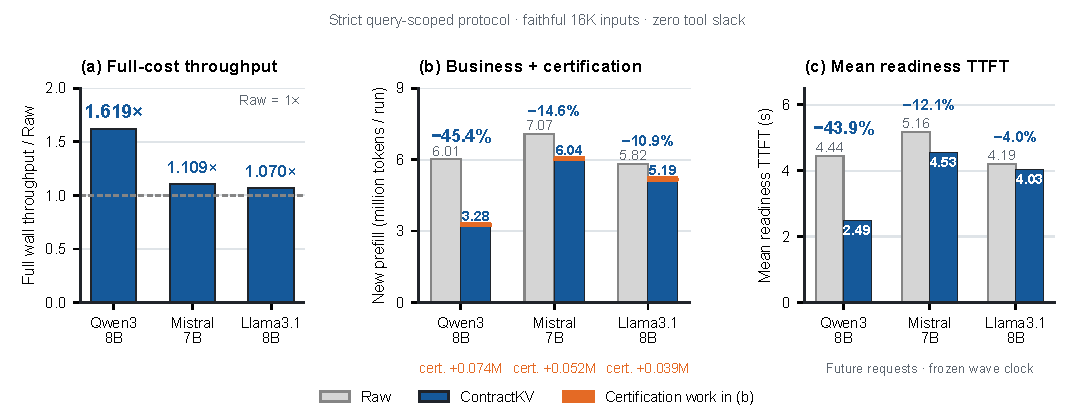
\includegraphics[width=\textwidth]{figures/fig2_full_cost_benefits.pdf}
\caption{Strict query-qualified performance on six source-disjoint HotpotQA/RepoBench templates, three processes/model, faithful 16K inputs, and zero slack. (a) Throughput charges all business responses, qualification, failed attempts, and synchronous waiting. (b) Actual business plus qualification new-prefill counts per run; orange caps mark certification work at its true scale, with exact added counts below. (c) Mean readiness TTFT over future requests uses the frozen two-request wave clock. Three-repeat values and tail statistics are reported separately.}
\label{fig:performance}
\end{figure*}

Figure~\ref{fig:performance}(b) measures the work saved: including qualification, total new-prefill counts fall by 45.44\%, 14.64\%, and 10.89\%. These scheduler observations are workload counts, not inferred GPU time. Directly measured mean readiness falls by 43.87\%, 12.09\%, and 3.99\%.

\begin{table}[t]
\centering\small
\caption{Tail cost and admitted coverage in the primary cohort. Readiness statistics concern future requests. Full process ranges and source-cluster intervals are in the supplement.}
\label{tab:primary}
\begin{tabular}{@{}lrr@{}}
\toprule
Model & Compiled / future pairs & p99 raw $\rightarrow$ CKV (ms)\\
\midrule
Qwen & 684 / 1,620 & 8,561.8 $\rightarrow$ 9,146.6\\
Mistral & 342 / 1,620 & 9,418.2 $\rightarrow$ 9,511.3\\
Llama & 270 / 1,620 & 7,851.3 $\rightarrow$ 7,905.7\\
\bottomrule
\end{tabular}
\end{table}

The throughput result does not imply lower tails. All p99 point estimates increase (Table~\ref{tab:primary}); Mistral's source-cluster/repetition interval for p99 reduction is wholly negative, [-60.576, -0.137]\%. Mean reduction intervals are [5.640, 79.479]\%, [-0.350, 34.781]\%, and [1.550, 5.724]\%. The cohort therefore supports a full-cost execution benefit with source-dependent latency effects.

A separate six-source Qwen cohort supplies an independent content check: unchanged ContractKV reaches 1.803$\times$ throughput (process range 1.798--1.808$\times$) and 774/1,620 compiled future pairs. It is a second cohort, not an additional model bar or another repetition of Fig.~\ref{fig:performance}.

\noindent\emph{Finding:} object-level admission can repay its measured cost under both declared regimes; the zero-slack task result does not depend on the deployment slack accounting.

\subsection{Does Qualification Preserve Observed Behavior?}
\label{sec:quality}
Compilation must obtain its gain within the admitted behavioral scope. Figure~\ref{fig:behavior} reports both scope coverage and free-running evidence. All 1,296 compiled future pairs have identical output IDs and unchanged scores. Including initial business rounds gives 1,440 compiled pairs with the same outcome. HotpotQA contributes compiled requests for every model; Qwen additionally admits RepoBench, whereas Mistral/Llama keep the inherited L0 route.

\begin{figure}[!t]
\centering
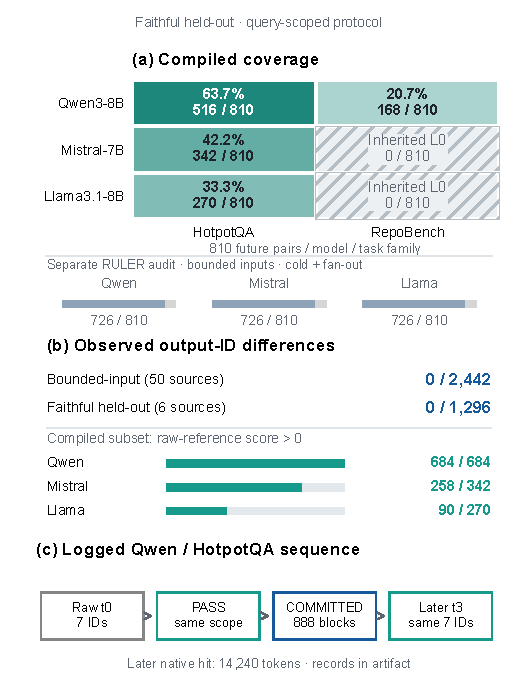
\includegraphics[width=\columnwidth]{figures/fig3_coverage_and_fidelity.pdf}
\caption{Qualification coverage and free-running evidence. (a) Each model/task cell has 810 future pairs; hatched cells inherit L0. The separate RULER strip uses bounded inputs and pooled cold/fan-out traces, not the faithful matrix protocol. (b) Output-ID differences and raw-reference positive-score counts within compiled subsets. Positive credit is not complete correctness. (c) One logged Qwen/HotpotQA witness, PASS, committed prefix and later identical output; full records are archived.}
\label{fig:behavior}
\end{figure}

Behavioral preservation and absolute utility remain different outcomes. Qwen's 684 admitted raw references all receive positive score credit; the counts are 258/342 for Mistral and 90/270 for Llama. Llama preserves 180 zero-F1 future references from two HotpotQA sources, and Mistral preserves 84 from one source. Neither exact agreement nor positive partial credit establishes semantic correctness.

Across all business routes, material score increases/decreases are 0/0 for Qwen, 2/1 for Mistral, and 5/3 for Llama. All changes occur on L0; the Mistral decrease is in an initial request and the Llama decreases are future requests. Corresponding output variants appear in scheduled raw-only repeats, demonstrating background variation, but not proving that every L0 event is unrelated to policy-associated execution conditions.

The bounded-input audit in Fig.~\ref{fig:behavior}(b) retains 2,442 compiled future pairs from a 50-source, five-family protocol: 2,178 RULER, 174 NarrativeQA, and 90 RepoBench~\cite{ruler2024,narrativeqa2018,qasper2021}. For RULER, each model contributes 726/810 admitted pairs (210/270 cold and 516/540 fan-out), shown separately from the main matrix. The complete bounded-input cohort has zero compiled ID changes and 33 full-route material decreases on L0. It uses fixed-cap packing and a mixed cold/fan-out trace, unlike the faithful main cohort. RULER supports that separate audit; it does not substitute for the common non-RULER evidence in panel (a).

\paragraph{Why the scope matters.}
A broad-wrapper development protocol admitted later wrappers and produced 108 material decreases among 3,672 compiled pairs. A Qwen NarrativeQA development case changed its raw answer under an allowed turn-field change while the compiled answer retained the witness, despite a 0.40625 candidate margin. The evaluated eligibility class was frozen before the independent sources were opened. A margin alone cannot justify extending evidence to unseen dynamic inputs.

\paragraph{Actual output horizon.}
Separate conditions produce and verify naturally terminated outputs of 642 tokens for Qwen, 769 for Mistral, and 578 for Llama, each with six correct future pairs across three processes. They use explicitly declared 128/128/192-item schemas. Llama's 224-item condition omits the final 100 items and remains a task failure. These results establish actual 512+ output conditions, not universal long-output correctness.

\noindent\emph{Finding:} admitted free-running behavior is preserved in the measured scopes, while coverage and absolute reference utility remain explicit.

\subsection{Does Governance Preserve the Service Benefit?}
\label{sec:ablation}
A frozen safe layout isolates available reuse, whereas governance should determine which candidates acquire shared visibility. Figure~\ref{fig:governance} examines both questions on deployment-qualified controls. D1 uses a prequalified layout without online registration; D2 adds verification and transactional registration. Native D0 delivers 0.066 requests/s at the 500-ms SLO; D1 and D2 deliver 1.472 and 1.428. D2 retains 97.0\% of the frozen layout's mean goodput while executing registration and publication: a 0.044 requests/s (3.0\%) mean reduction relative to D1. Their TTFTs are 194.95 and 194.72 ms. D0 supplies the absolute service reference; D1 isolates the available layout benefit.

\begin{figure}[!t]
\centering
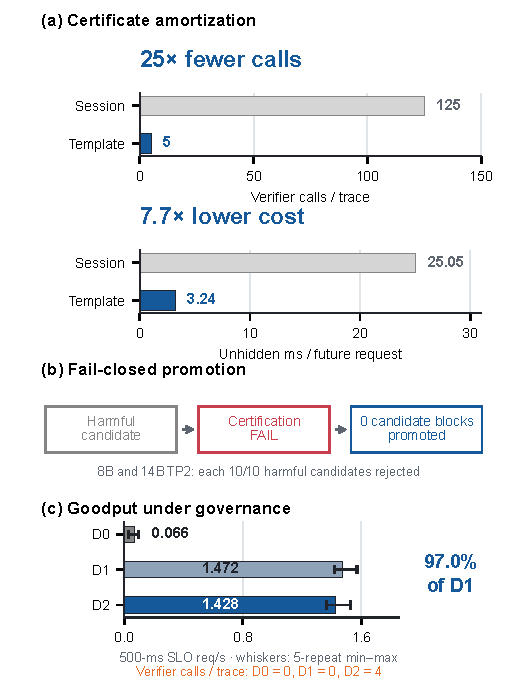
\includegraphics[width=\columnwidth]{figures/fig4_transaction_and_amortization.pdf}
\caption{Separate deployment controls. (a) Registration granularity with fixed layout/locality; three processes and 1,125 future requests/trace. (b) Each 8B/14B TP2 probe rejects 10/10 harmful candidates with zero rejected-candidate promotion. (c) Same-engine D0/D1/D2 500-ms SLO goodput; whiskers are five-process min--max, not confidence intervals.}
\label{fig:governance}
\end{figure}

Behaviorally harmful, dependency-valid candidates provide the complementary test. In each of two controlled 20-case sets, all ten harmful candidates are rejected with zero newly promoted candidate tokens. A 14B control also checks actual post-decision outputs against raw scores. Live source-hook, concurrency, cancellation, duplicate, timeout, and authenticated-binding controls exercise the publication boundary. The separate 325,000-operation stress study tests the in-memory state machine and is not counted as GPU serving evidence.

\subsubsection{The unit of amortization}
\label{sec:deployment}
The fixed-layout amortization in Section~\ref{sec:mainresults} changes the registration unit rather than the physical layout: prefix hits remain 97.82\%/98.19\%. Template identity therefore lets the platform share the evidence cost without surrendering the qualification or publication boundary.

Query-qualified execution has a different amortization unit. The second Qwen cohort obtains 774 compiled future pairs from 27 issued scope-repeat decisions and 42 total GPU calls, including failures. Its cost grows with distinct selected scopes, then amortizes across tenants using them. This preserves the template prefix as the physical object without assigning deployment's $O(1)$ behavioral cost to arbitrary dynamic queries.

\begin{figure}[!t]
\centering
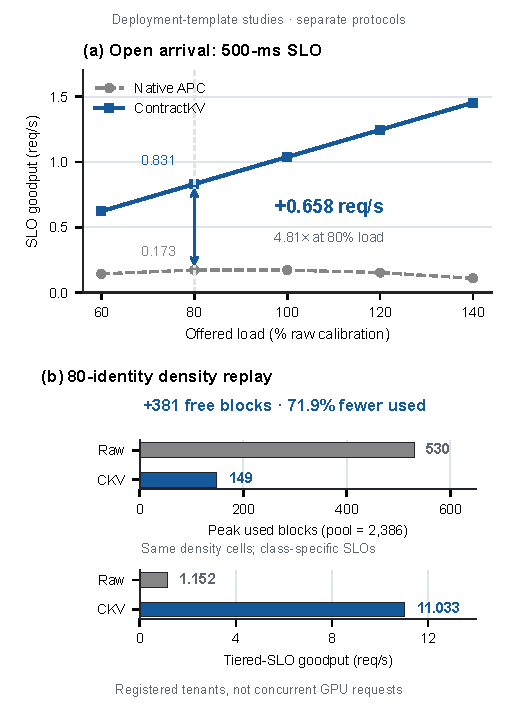
\includegraphics[width=\columnwidth]{figures/fig5_service_goodput_and_kv_savings.pdf}
\caption{Distinct deployment protocols. (a) Open-arrival 500-ms SLO goodput; the 4.81$\times$ ratio is the 80\%-load point. (b) The same 80-identity density cells supply both allocator occupancy and goodput under class-specific 750/1,500/3,000-ms SLOs, with a 2,386-block pool. Registered identities are not simultaneous GPU requests.}
\label{fig:service}
\end{figure}

Figure~\ref{fig:service} tests a separately qualified deployment workload at fixed arrival loads and in bounded-concurrency density replay. At 25 tenants per template and 80\% calibrated arrival load, 500-ms goodput rises 0.173 to 0.831 requests/s. The density experiment then tests whether the shared object remains useful as authorized fan-out increases. Across 10--80 registered identities, ContractKV sustains 9.408--11.072 tiered-SLO requests/s, compared with 0.900--1.152 for native APC (Supplementary Table~S-III). At 80 identities, used blocks decrease by 71.9\%, leaving 381 more free blocks. Density goodput and block values come from the same cells, but do not isolate headroom as the sole cause of improved throughput. These marker-bearing service traces have a separate task-quality audit and are distinct from the task-bearing primary cohort.

\noindent\emph{Finding:} publication governance retains the frozen layout's service benefit, and the template object supports measurable cost sharing and physical consolidation across tenants.

\subsection{What Determines the Operating Region?}
\label{sec:residency}
\begin{figure}[!t]
\centering
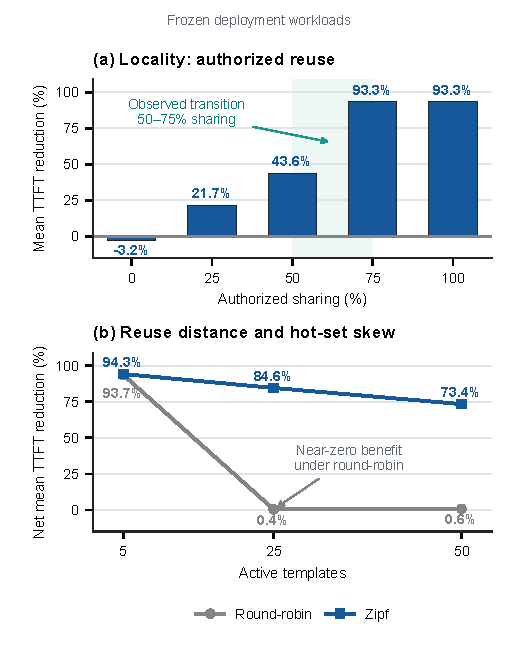
\includegraphics[width=\columnwidth]{figures/fig6_locality_and_residency.pdf}
\caption{Operating region in frozen deployment workloads. (a) The shaded 50--75\% sharing interval is an observed transition, not a universal threshold. (b) Access-pattern sensitivity to reuse distance and hot-set skew. Both axes report TTFT reduction; neither is a direct residency fraction.}
\label{fig:region}
\end{figure}

The object pays off when authorized reuse is sufficiently dense and its physical state remains available. Figure~\ref{fig:region} varies these conditions with a frozen deployment workload. Benefit rises sharply over an observed sharing interval, but round-robin access to a larger working set nearly eliminates it. A qualified object still needs resident physical blocks. In the primary cohort, 189 compiled business requests have incomplete hits: 135 Llama zero hits, 42 Mistral zero hits, and 12 Qwen partial hits. All 1,440 compiled business requests match the certified prefix IDs and commit boundary; each incomplete-hit request has a later full-hit peer in its two-request wave.

To test the physical cause, three frozen known-source probes replay archived IDs with read-only instrumentation of lookup, publication, and reclamation. Across 138 business requests and four successful qualifications, all 13 incomplete hits follow deletion of the last matching native mapping at reference count zero. Salt and hash chains match the certificate, while the mapping is absent before lookup. All 12 immediate post-commit reuse controls fully hit. These events match the native cache reclamation design~\cite{vllmAPC}. They diagnose the three sources, not every historical event, and do not supply a new performance number. Figure~\ref{fig:performance} already charges misses and recomputation.

\begin{table}[t]
\centering\small
\caption{Four sealed operating points under the development-frozen benefit gate. Net benefit is per certificate; rejected points serve raw. Candidate diagnostics were also run for rejected points, so this table does not measure avoided online verifier calls.}
\label{tab:gate}
\begin{tabular}{@{}rrrrr@{}}
\toprule
Prefix & Uses & Slack (s) & Route & Net benefit (s)\\
\midrule
1500 & 8 & 3.5 & Raw & 0.00\\
3000 & 12 & 0.5 & CKV & 7.04\\
5000 & 10 & 1.5 & CKV & 10.84\\
3500 & 6 & 6 & Raw & 0.00\\
\bottomrule
\end{tabular}
\end{table}


The frozen benefit gate selects two of four sealed points (Table~\ref{tab:gate}); both selected points are net-positive at 7.04 and 10.84 s/certificate. Rejected points serve raw, while their candidate outcomes remain diagnostics. This validates the declared operating-point rule, not a learned predictor or a claim that diagnostic verifier work was avoided.

\label{sec:costvariant}
A separate length-aware waiting-budget variant illustrates the cost of overly narrow profiling support. On an independent Qwen cohort it lowers p99 from 13,386.9 to 8,801.9 ms but removes useful scopes: compiled coverage falls 774 to 258 pairs and throughput 1.803$\times$ to 1.070$\times$. The source/repetition interval for p99 reduction crosses zero. Full development and independent results, including all L0 variations, remain in the supplement; the original query-qualified gate is retained for the main measurements.

\noindent\emph{Finding:} scope determines admissible sharing, and locality, residency and admission cost determine how much of that opportunity becomes service benefit.

\subsection{How Does Input Structure Affect Reuse?}
\label{sec:fidelity}
Preserving task-critical fields should improve the usefulness of both raw execution and any behavior it can qualify. A same-source four-cell Qwen experiment compares fixed-word-cap, whitespace-normalized packing with structure-preserving rendering on two HotpotQA and two RepoBench sources. Window, two-request concurrency, admission, scoring and service clock stay fixed.

Raw HotpotQA F1 rises from 0 to 0.22222 and code score from 0.12067 to 0.36667. Admitted coverage rises from 30/360 to 112/360 and full-wall throughput from 1.039$\times$ to 1.117$\times$, with unchanged compiled IDs. These are input-construction effects, not accuracy gains caused by reordering. The supplement records content retention, code-prefix loss and whitespace effects. The independent primary cohort tests the structure-preserving pipeline without changing its acceptance rules.

\noindent\emph{Finding:} input fidelity changes both absolute task utility and the reuse that can be admitted, so task construction belongs in a cache-system evaluation.

\subsection{What Does Matched-Native Comparison Establish?}
\label{sec:baselines}
Cross-position methods require their own matched-native references. A 9,000-pair quality study has 2,250 pairs/method: CacheBlend records 224 material decreases and 331 increases, with mean score 0.333210$\rightarrow$0.339817; ContractKV records two decreases and no increases, with 0.353780$\rightarrow$0.353744. Different raw means, runtimes, prompt construction, and separators preclude a direct speed ranking or multiplicative causal risk claim. Supplementary Table~S-VIII restores all four methods, both change directions and their own reference means; threshold sensitivity remains in the source tables. Mean task utility and per-request behavioral preservation answer different questions; same-engine D1/D2 supplies the performance attribution.

\noindent\emph{Finding:} mean utility and per-request preservation answer different questions; comparisons must retain each system's own execution reference.
